\documentclass[crop]{standalone}

\usepackage[lite,subscriptcorrection,slantedGreek,nofontinfo]{mtpro2}
\usepackage{amsmath}
\usepackage{amsfonts}
\usepackage{amssymb}
\usepackage{bm}

\usepackage{tikz}
\usetikzlibrary{calc}
\usetikzlibrary{arrows.meta, datavisualization.formats.functions, positioning, fpu, calc, bending, perspective}

\begin{document}

\pagestyle{empty}

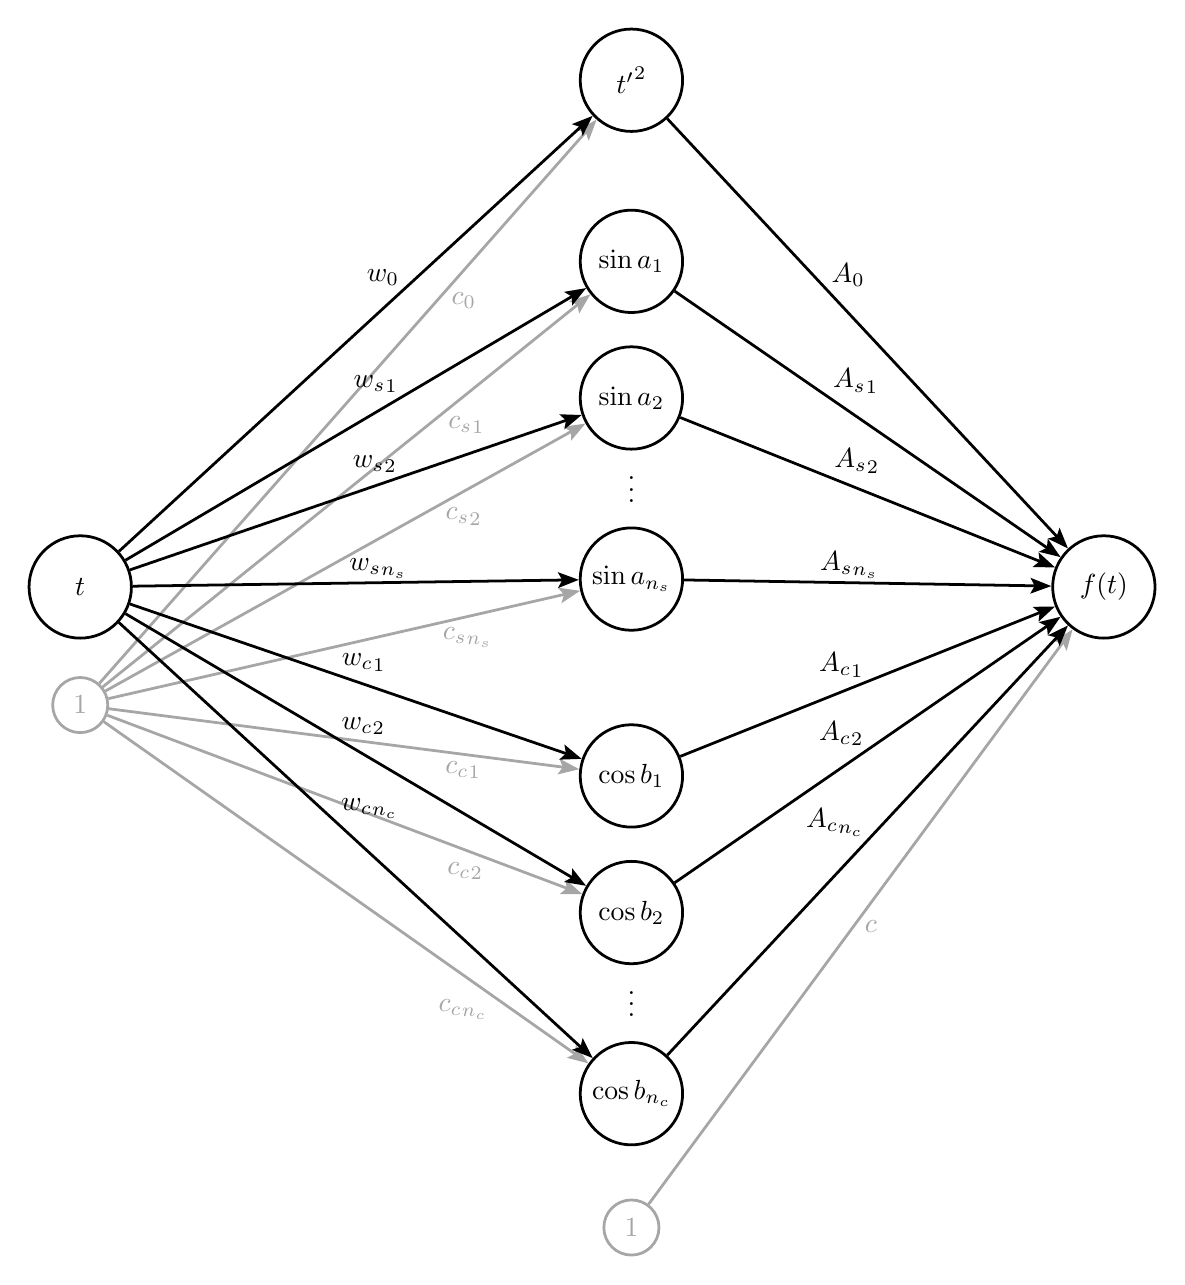
\begin{tikzpicture}[every edge/.style={draw,->,line width=1pt, arrows={-Stealth[inset=1.5pt]}, auto}]%
	
	\begin{scope}[every node/.style={draw, node distance=0.4cm and 1.5cm, circle, line width=1pt, minimum size=1.3cm, inner sep=0pt, text width=1cm, align=center}]
		
		\node (t2) {${t'}^2$};
		
		\node (sin1) at ($(t2) + (0cm,-2.3cm)$) {$\sin a_1$};
		\node (sin2) [below=of sin1] {$\sin a_2$};
		\node (sinns) at ($(sin2) + (0cm,-2.3cm)$) {$\sin a_{n_s}$};
		\node[draw=none] (dots1) at ($(sin2)!.46!(sinns)$) {$\vdots$};
		
		\node (cos1) at ($(sinns) + (0cm,-2.5cm)$) {$\cos b_1$};
		\node (cos2) [below=of cos1] {$\cos b_2$};
		\node (cosnc) at ($(cos2) + (0cm,-2.3cm)$) {$\cos b_{n_c}$};
		\node[draw=none] (dots2) at ($(cos2)!.46!(cosnc)$) {$\vdots$};
		
		\node (t) at ($(t2)!.5!(cosnc) + (-7cm, 0cm)$) {$t$};
		\node (f) at ($(t2)!.5!(cosnc) + (6cm, 0cm)$) {$f(t)$};
	\end{scope}
	
	\node[draw, circle, line width=1pt, minimum size=0.7cm, color=gray!70] (b1) at ($(t) + (0cm, -1.5cm)$) {$1$};
	\draw (b1) edge[color=gray!70, swap] node[pos=0.7, inner sep=1pt, color=gray!70] {$c_0$} (t2);
	\draw (b1) edge[color=gray!70, swap] node[pos=0.7, inner sep=1pt] {${c_s}_1$} (sin1);
	\draw (b1) edge[color=gray!70, swap] node[pos=0.7, inner sep=1pt] {${c_s}_2$} (sin2);
	\draw (b1) edge[color=gray!70, swap] node[pos=0.7, inner sep=1pt] {${c_s}_{n_s}$} (sinns);
	\draw (b1) edge[color=gray!70, swap] node[pos=0.8, inner sep=1pt] {${c_c}_1$} (cos1);
	\draw (b1) edge[color=gray!70, swap] node[pos=0.8, inner sep=1pt] {${c_c}_2$} (cos2);
	\draw (b1) edge[color=gray!70, swap] node[pos=0.8, inner sep=1pt] {${c_c}_{n_c}$} (cosnc);
	
	\node[draw, circle, line width=1pt, minimum size=0.7cm, color=gray!70] (b2) at ($(cosnc) + (0cm,-1.7cm)$) {$1$};
	\draw (b2) edge[color=gray!70, swap] node[midway, inner sep=1pt] {${c}$} (f);	
	
	\draw (t) edge node[pos=0.6, inner sep=1pt] {$w_0$} (t2);
	\draw (t) edge node[pos=0.6, inner sep=1pt] {${w_s}_1$} (sin1);
	\draw (t) edge node[pos=0.6, inner sep=1pt] {${w_s}_2$} (sin2);
	\draw (t) edge node[pos=0.55, inner sep=1pt] {${w_s}_{n_s}$} (sinns);
	\draw (t) edge node[pos=0.46, inner sep=1pt] {${w_c}_1$} (cos1);
	\draw (t) edge node[pos=0.46, inner sep=1pt] {${w_c}_2$} (cos2);
	\draw (t) edge node[pos=0.46, inner sep=1pt] {${w_c}_{n_c}$} (cosnc);
	
	\draw (t2) edge node[pos=0.4, inner sep=1pt] {$A_0$} (f);
	\draw (sin1) edge node[pos=0.4, inner sep=1pt] {${A_s}_1$} (f);
	\draw (sin2) edge node[pos=0.4, inner sep=1pt] {${A_s}_2$} (f);
	\draw (sinns) edge node[pos=0.45, inner sep=1pt] {${A_s}_{n_s}$} (f);
	\draw (cos1) edge node[pos=0.5, inner sep=1pt] {${A_c}_1$} (f);
	\draw (cos2) edge node[pos=0.5, inner sep=1pt] {${A_c}_2$} (f);
	\draw (cosnc) edge node[pos=0.5, inner sep=1pt]	 {${A_c}_{n_c}$} (f);
\end{tikzpicture}

\end{document}
